\documentclass[12pt]{article}
\usepackage{fancyhdr}
\usepackage{parskip}
\usepackage{graphicx}
\lhead{CSC 428A: Sudoku Puzzles}
\rhead{Samuel Maskell \thepage}
\fancyfoot{}
\title{Generating and Solving Sudoku Puzzles using DLX and SAT Solvers\\CSC 428A - Spring 2014}
\date{April 23, 2014}
\author{Samuel Maskell\\ V00700592}

\usepackage{tikz}
\usepackage{mathpazo}
%\usepackage[pdftex,active,tightpage]{preview}
%\PreviewEnvironment{tikzpicture}
\newcounter{row}
\newcounter{col}

\newcommand\setrow[9]{
  \setcounter{col}{1}
  \foreach \n in {#1, #2, #3, #4, #5, #6, #7, #8, #9} {
    \edef\x{\value{col} - 0.5}
    \edef\y{9.5 - \value{row}}
    \node[anchor=center] at (\x, \y) {\n};
    \stepcounter{col}
  }
  \stepcounter{row}
}

\usepackage{amsmath}
\usepackage{algorithm}
\usepackage[noend]{algpseudocode}
\renewcommand{\algorithmicforall}{\textbf{for each}}
\begin{document}
\begin{titlepage}
\maketitle
\thispagestyle{empty}
\end{titlepage}
\pagestyle{fancy}
\section{The Game of Sudoku}
The game of Sudoku involves a 9 by 9 grid made up for nine 3 by 3 sub-grids, often referred to as blocks. Initially, certain cells contain a digit between 1 and 9 while others are left blank. The objective of the game is to fill in the remaining cells in such a way that each number between 1 and 9 appears exactly once in every row, every column, and every block. This can be accomplished using a variety of techniques to infer the possible candidates for a given cell, removing possibilities until only one remains. However, in the case of a computer, it is generally simpler to apply a simple backtracking technique. \\


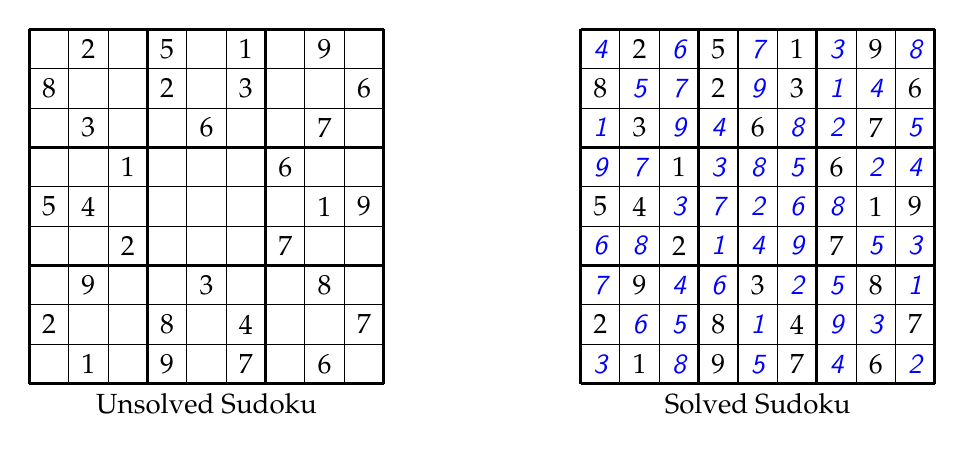
\begin{tikzpicture}[scale=.5]

  \begin{scope}[xshift=-2cm]
    \draw (0, 0) grid (9, 9);
    \draw[very thick, scale=3] (0, 0) grid (3, 3);

    \setcounter{row}{1}
    \setrow { }{2}{ }  {5}{ }{1}  { }{9}{ }
    \setrow {8}{ }{ }  {2}{ }{3}  { }{ }{6}
    \setrow { }{3}{ }  { }{6}{ }  { }{7}{ }

    \setrow { }{ }{1}  { }{ }{ }  {6}{ }{ }
    \setrow {5}{4}{ }  { }{ }{ }  { }{1}{9}
    \setrow { }{ }{2}  { }{ }{ }  {7}{ }{ }

    \setrow { }{9}{ }  { }{3}{ }  { }{8}{ }
    \setrow {2}{ }{ }  {8}{ }{4}  { }{ }{7}
    \setrow { }{1}{ }  {9}{ }{7}  { }{6}{ }

    \node[anchor=center] at (4.5, -0.5) {Unsolved Sudoku};
  \end{scope}

  \begin{scope}[xshift=12cm]
    \draw (0, 0) grid (9, 9);
    \draw[very thick, scale=3] (0, 0) grid (3, 3);

    \setcounter{row}{1}
    \setrow { }{2}{ }  {5}{ }{1}  { }{9}{ }
    \setrow {8}{ }{ }  {2}{ }{3}  { }{ }{6}
    \setrow { }{3}{ }  { }{6}{ }  { }{7}{ }

    \setrow { }{ }{1}  { }{ }{ }  {6}{ }{ }
    \setrow {5}{4}{ }  { }{ }{ }  { }{1}{9}
    \setrow { }{ }{2}  { }{ }{ }  {7}{ }{ }

    \setrow { }{9}{ }  { }{3}{ }  { }{8}{ }
    \setrow {2}{ }{ }  {8}{ }{4}  { }{ }{7}
    \setrow { }{1}{ }  {9}{ }{7}  { }{6}{ }

    \node[anchor=center] at (4.5, -0.5) {Solved Sudoku};

    \begin{scope}[blue, font=\sffamily\slshape]
      \setcounter{row}{1}
      \setrow {4}{ }{6}  { }{7}{ }  {3}{ }{8}
      \setrow { }{5}{7}  { }{9}{ }  {1}{4}{ }
      \setrow {1}{ }{9}  {4}{ }{8}  {2}{ }{5}

      \setrow {9}{7}{ }  {3}{8}{5}  { }{2}{4}
      \setrow { }{ }{3}  {7}{2}{6}  {8}{ }{ }
      \setrow {6}{8}{ }  {1}{4}{9}  { }{5}{3}

      \setrow {7}{ }{4}  {6}{ }{2}  {5}{ }{1}
      \setrow { }{6}{5}  { }{1}{ }  {9}{3}{ }
      \setrow {3}{ }{8}  { }{5}{ }  {4}{ }{2}
    \end{scope}

  \end{scope}

\end{tikzpicture} \\

Given the nature of the problem, solving Sudoku puzzles can easily be modelled as many different constraint satisfaction problems, such as exact cover or boolean satisfiability. In doing so, standard techniques for solving these well known problems can be applied rather than creating a customized solution.  \\

\section{Sudoku as an Exact Cover Problem}
Given a binary matrix, the exact cover problem is to find a set of rows such that there is a 1 in every column in exactly one of the rows in the set. Typically, the columns are used to represent constraints that must be satisfied. Each row in the matrix represents a partial solution, with conflicting partials solutions containing in the same column of their rows for the rule(s) on which they conflict. \\

Sudoku has four types of constraints
\begin{description}
\item[Cell Constraints] Each cell must have exactly one number in it
\item[Row Constraints] Each row much contain each number exactly once
\item[Column Constraints] Each column much contain each number exactly once
\item[Block Constraints] Each block much contain each number exactly once
\end{description}
As such, the base set of constraints result in $4*9*9$ columns; there is a cell constraint for each of the 81 cells and there is a row, column and block constraint for each number in each row, column or block. Furthermore, there are $9*9*9$ rows, one for each number in each cell. The rows have 1's in the columns for the constraints that they satisfy. \\

Once the initial constraints have been set up, the columns all of the constraints which are satisfied by any of given cells in a puzzle can be removed, as well as all rows that could have satisfied any of those constraints. The remaining columns will be those which need to be satisfied in order to complete the puzzle and the rows will be the possible options.
\section{Algorithm X and Dancing Links}
In his paper, "Dancing Links", Donald Knuth describes an algorithm for solving the exact cover problem, which he calls Algorithm X, and a possible implementation technique, which he calls dancing links. This implementation is often referred to as DLX for short. \\
The dancing links approach is based on the observation that an element, x, in a doubly linked list can be removed in the following manner
\[ x.left.right \gets x.right, x.right.left \gets x.left \]
and, more interestingly, x can be re-inserted into the list thusly
\[ x.left.right \gets x, x.right.left \gets x \]
\\
The matrix of the exact cover problem can be represented as a 2-dimensional, circular linked list with a node for every 1 in the matrix, with every node having up, down, left and right pointers. Knuth also uses a set of column header nodes that keep track of additional information about a given column as well as a special \textit{h} node that simply points to the top of the first column. Furthermore, every node has a reference to its column header. This is data structure is shown in Figure~\ref{dlx}. In the figure, the columns are labelled A through G and the numbers below the labels simply refer the number of rows in that column.
\begin{figure}[!ht]
\begin{center}
\includegraphics[width=0.9\columnwidth]{dancing_links}
\caption{DLX data structure}
\label{dlx}
\end{center}
\end{figure}
Given this data structure, it is very easy to remove columns and rows, as well as to add them back in again, using the approach described above. The only constraint is that the columns/rows must be added back in in the opposite order from which that in which they were removed. With this in mind, Algorithm X becomes quite simple. \\ 
\begin{algorithm}
\caption{DLX}\label{search}
\begin{algorithmic}[1]
\Procedure{Search}{h: Node}
\If {$h.right = h$}
\State print \textit{solution}
\State \Return
\EndIf
\State $col \gets$ \Call{chooseNextColumn}{$h$}
\State \Call{cover}{$col$}
\ForAll{$row \gets col.down, col.down.down, \dots, while\ row \neq col$}
\State add $row$ to current solution
\ForAll{$j \gets row.right, row.right.right,\dots, while\ j \neq row$}
\State \Call{cover}{$j.colHeader$}
\EndFor
\State \Call{search}{$h$}
\ForAll{$j \gets row.left, row.left.left,\dots, while\ j \neq row$}
\State \Call{uncover}{$j.colHeader$}
\EndFor
\State remove $row$ from the current solution
\EndFor
\State \Call{uncover}{$col$}
\EndProcedure
\end{algorithmic}
\end{algorithm}


The idea is quite simple; we select a column that we want to satisfy and remove it and then, for each row that satisfies the chosen column, we try removing it and all other columns that it satisfies and then we recurse. When the recursion completes, we must undo what we have done so far before we move on to the next candidate row. \\ 

The order in which the columns are chosen does not affect the final result. However, the amount of branching can be reduced if the column with the fewest number of rows is selected at each step. \\

The operation of ``covering'' is also fairly straight forward. We must simply remove the column header from list, so that it will not be chosen later, and then all the rows in the column from all other columns in which they appear. Uncovering, of course, is simply the exact opposite, done in reverse order. \\

\begin{algorithm}
\label{cover}
\begin{algorithmic}
\Procedure{Cover}{col: Node}
\State $col.right.left \gets col.left$
\State $col.left.right \gets col.right$
\ForAll{$row \gets col.down, col.down.down, \dots, while\ row \neq col$}
\ForAll{$j \gets row.right, row.right.right,\dots, while\ j \neq row$}
\State $j.up.down \gets j.down$
\State $j.down.up \gets j.up$
\State $j.colHeader.size \gets j.colHeader.size - 1$
\EndFor
\EndFor
\EndProcedure
\end{algorithmic}
\end{algorithm}

\begin{algorithm}
\label{uncover}
\begin{algorithmic}
\Procedure{uncover}{col: Node}
\ForAll{$row \gets col.up, col.up.up, \dots, while\ row \neq col$}
\ForAll{$j \gets row.left, row.left.left,\dots, while\ j \neq row$}
\State $j.up.down \gets j$
\State $j.down.up \gets j$
\State $j.colHeader.size \gets j.colHeader.size + 1$
\EndFor
\EndFor
\State $col.right.left \gets col$
\State $col.left.right \gets col$
\EndProcedure
\end{algorithmic}
\end{algorithm}

\end{document}